%%%%%%%%%%%%%%%%%%%%%%%%%%%%%%%%%%%%%%%%%%%%%%%%%%%%%%%
%                   File: OSAmeetings.tex             %
%                  Date: March 21, 2007  MSD          %
%                                                     %
%     For preparing LaTeX manuscripts for submission  %
%       submission to OSA meetings and conferences    %
%                                                     %
%       (c) 2007 Optical Society of America           %
%%%%%%%%%%%%%%%%%%%%%%%%%%%%%%%%%%%%%%%%%%%%%%%%%%%%%%%

\documentclass[letterpaper,10pt]{article}
\usepackage{osameet2}

%% standard packages and arguments should be modified as needed

%%\usepackage{amsmath,amssymb}
\usepackage{indentfirst}
\setlength{\parindent}{2em}
    

%\usepackage[pdftex,colorlinks=true,bookmarks=false,citecolor=blue,urlcolor=blue]{hyperref} %pdflatex
\usepackage[dvips,colorlinks=false,bookmarks=false,citecolor=blue,urlcolor=blue]{hyperref} %latex w/dvips

\begin{document}
\title{Experimental Study of Co-propagation of Quantum and Optical Signals with Flattened and Spectrum-flexible Switching Node}
\author{Pandeng Li\thanks{Pandeng}, Yongmei Sun\thanks{Yongmei}, Jianing Niu\thanks{Jianing} and Yuefeng Ji\thanks{Yuefeng}}
%%\author{Yongmei Sun}
%%\author{Jianing Niu}
%%\author{Yuefeng Ji}
%% 
\address{State Key Laboratory of Information Photonics and Optical Communications, School of Information and Telecommunication Engineering, BUPT Beijing, China, 100876}
\email{ymsun@bupt.edu.cn}

\begin{abstract}
We demonstrate co-propagation of quantum and optical signals with flattened and spectrum-flexible switching node that could combine quantum-key-communication(QKD) network with optical network. It is multi-granularity and has the flexibility of spectrum and bandwidth allocation.
\end{abstract}
\ocis{(060.5565)Quantum communications, (060.2330)Fiber optics and optical communications}

\section{Introduction}

Quantum key distribution provides an unconditional physical layer for secure communication with using non-orthogonal coded single photon states such as single photon polarization, phase and angular momentum. These all can be transmitted and switched as same as optical signal. Since point-to-point co-fiber transmission for QKD communication has been quite mature, more and more researchers turned to studying large-scale and multi-user QKD network based on optical network. In 2010, \cite{Peters} demonstrated coexistence of classical and quantum signals for quantum key distribution in a DWDM reconfigurable network using a ROADM, but it has static allocation of resources. In 2016, \cite{YongmeiSun} proposed a unequal frequency spacing (UFS-iWDM) frequency allocation to reduce four-wave mixing(FWM) noise that falls at the quantum channels, this improves the performance of co-propagation. This paper will present an flattened switching node scheme supporting the co-propagation of quantum signal and optical signal. The node is based on WSS and coupler and could provide abilities of flexible spectrum allocation and non-blocking switching.

\section{Flattened and spectrum-flexible switching node based on WSS}

To combine QKD with optical communication, we should know features of both quantum signal and classic signal. The quantum signal can't be amplified, it needs the link loss to be extremely low, while the classic signal is not sensitive to the link loss. When passing through the beam splitter, quantum signal only appears in one branch of the beam splitter(BS) at a specific probability, while classic signal appears in all branchs of the BS at a specific ratio of the input power. In the process of QKD, the delay time between quantum signal and synchronization signal has an important effect on key generation rates. The synchronization signal is needed to have the same path with quantum signal on the link layer to keep the signal synchronized. Meanwhile,quantum signal is extremely weak and very easy to be disturbed by classic signals of other channels, so it's very important to consider the effects of classic signals on quantum signals when they are co-propagated. Luckly, WSS could meet all these requirements. The switching node structure based WSS and coupler is showed in figure \ref{Fig:switching_node_structure}.

\begin{figure}[htbp]
  \centering
  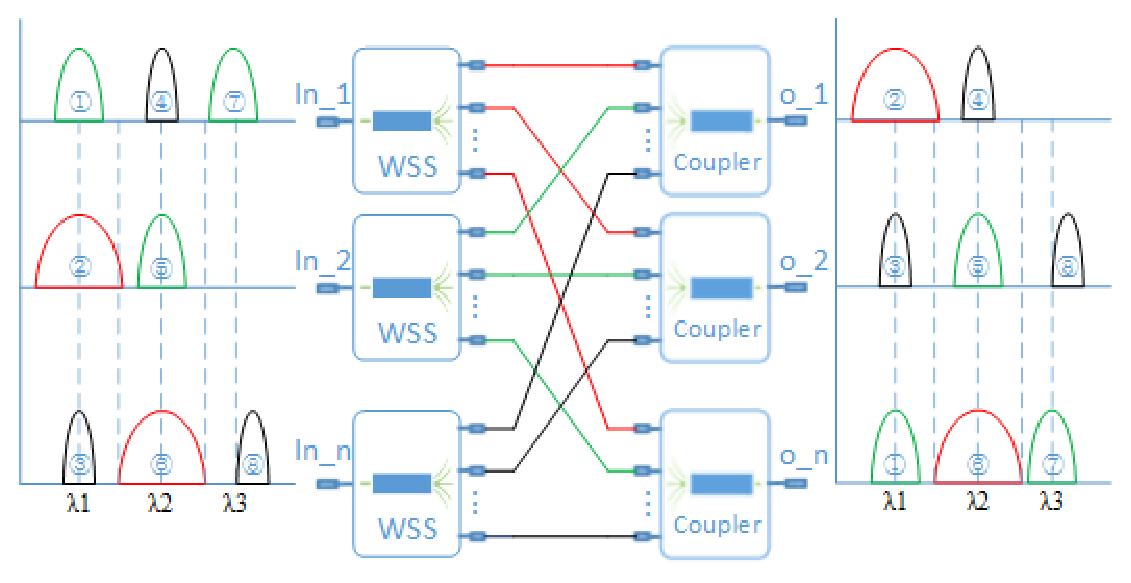
\includegraphics[width=8.3cm]{swtiching_node_struct}
  \caption{Switching Node Structure.} \label{Fig:switching_node_structure}
\end{figure}
Switching node has characteristics such as flexible grid, multi-granularity, low loss and non-blocking. So it could switch signal with variety of bandwidth simultaneously and could achieve 'Packet Routing' that the signals, who have the same destination but different wavelength and bandwidth, could always passing through the same classic fiber path. Based on this switching node, we could also design a wavelength allocation algorithm to reduce the impairment on the quantum channels induced by four-wave mixing (FWM). When expanding node's degree, it doesn't increase the device cascade. Therefore it's attenuation remains stable, approximately 3.5dB under current technical conditions. 

For classic signal, there is only one constraint that the signals couldn't overlap in the spectrum when they are switched to the same port. In figure \ref{Fig:switching_node_structure}, wave 2 and wave 6 have different center wavelengths, but their spectra have a little intersection, so they can't be switched to the same port. For quantum signal, we could compute the channels that FWM sit on according to the current classic signal passing the node, and make quantum signal stay away from these channels to reduce the interference induced by FWM when allocating the quantum signal channel. In the past studies, someone has proposed switching node based on WDM and OXC, and multi-granularity switching node of three-layers based on DWDM, CWDM and OXC. The comparisons of these three structures in figure \ref{Fig:loss_of_insertion} and \ref{Fig:distance_vs_qber} show that the flattened switching node we build has lower loss and greater transmission distance.

\begin{figure}[!htb]
   \begin{minipage}{0.48\textwidth}
     \centering
     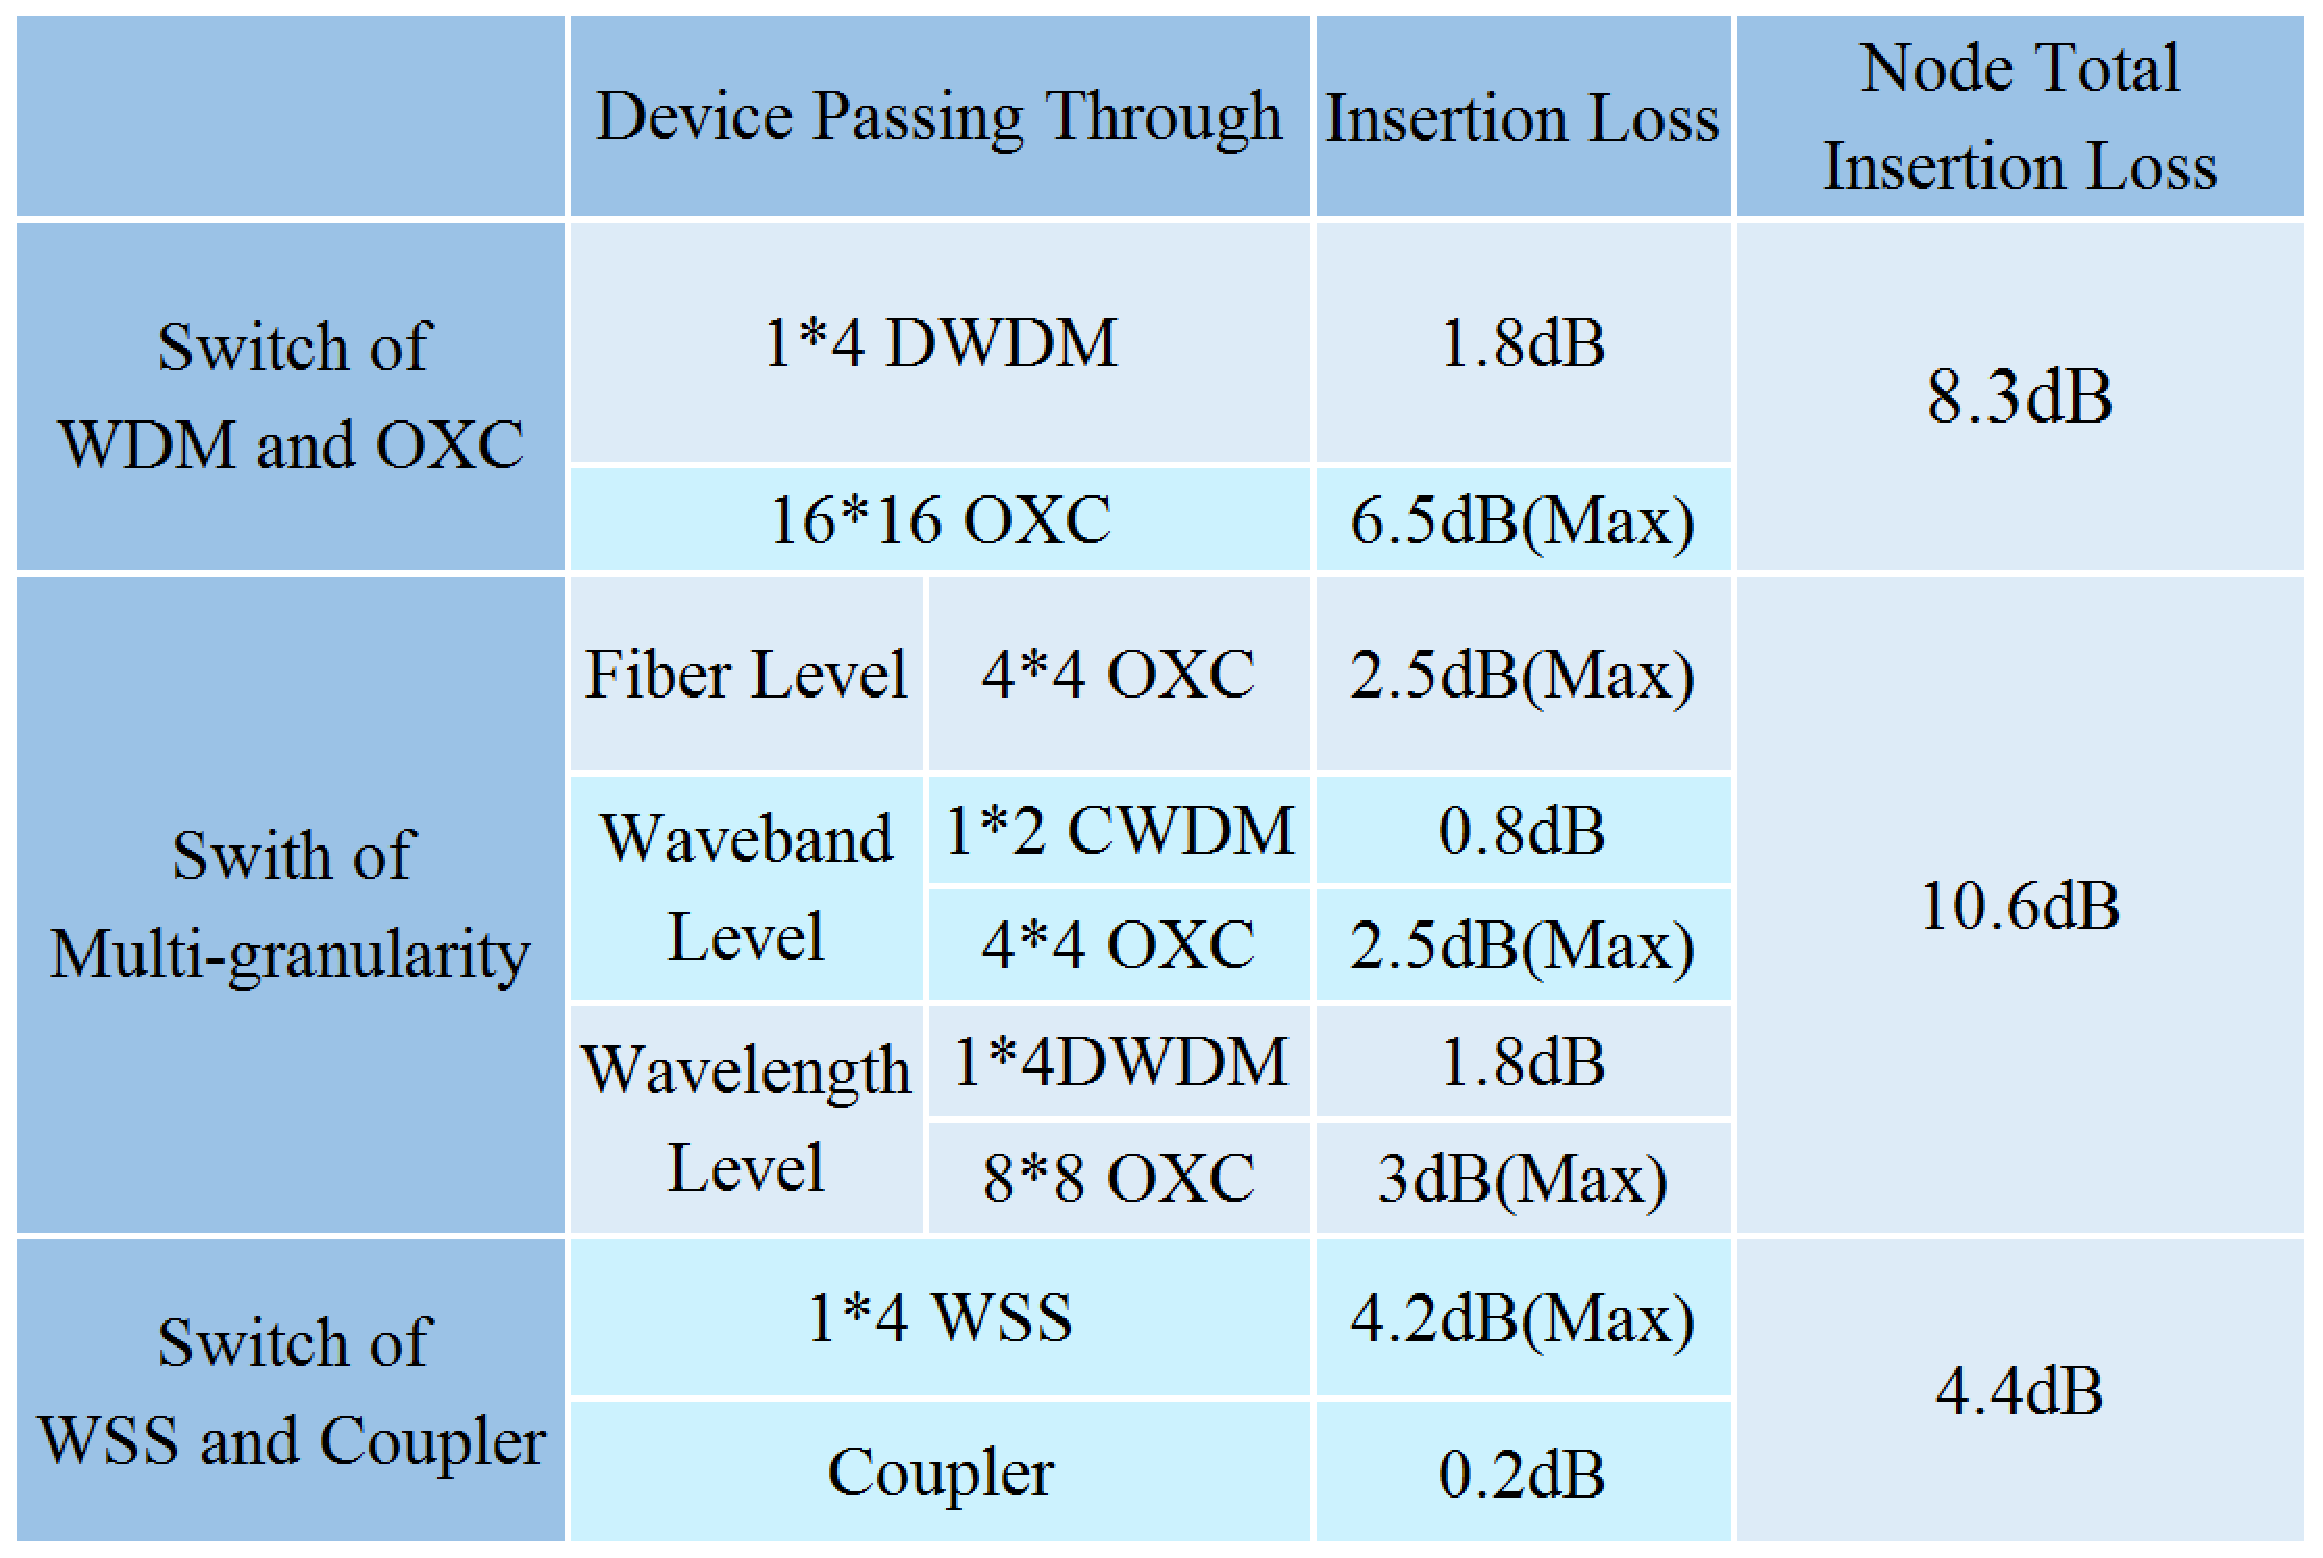
\includegraphics[height= 4cm,width=.9\linewidth]{comparison_of_three_kind_of_nodes_prety}
     \caption{Comparison of Insertion Loss} 
     \label{Fig:loss_of_insertion}
   \end{minipage}\hfill
   \begin{minipage}{0.48\textwidth}
     \centering
     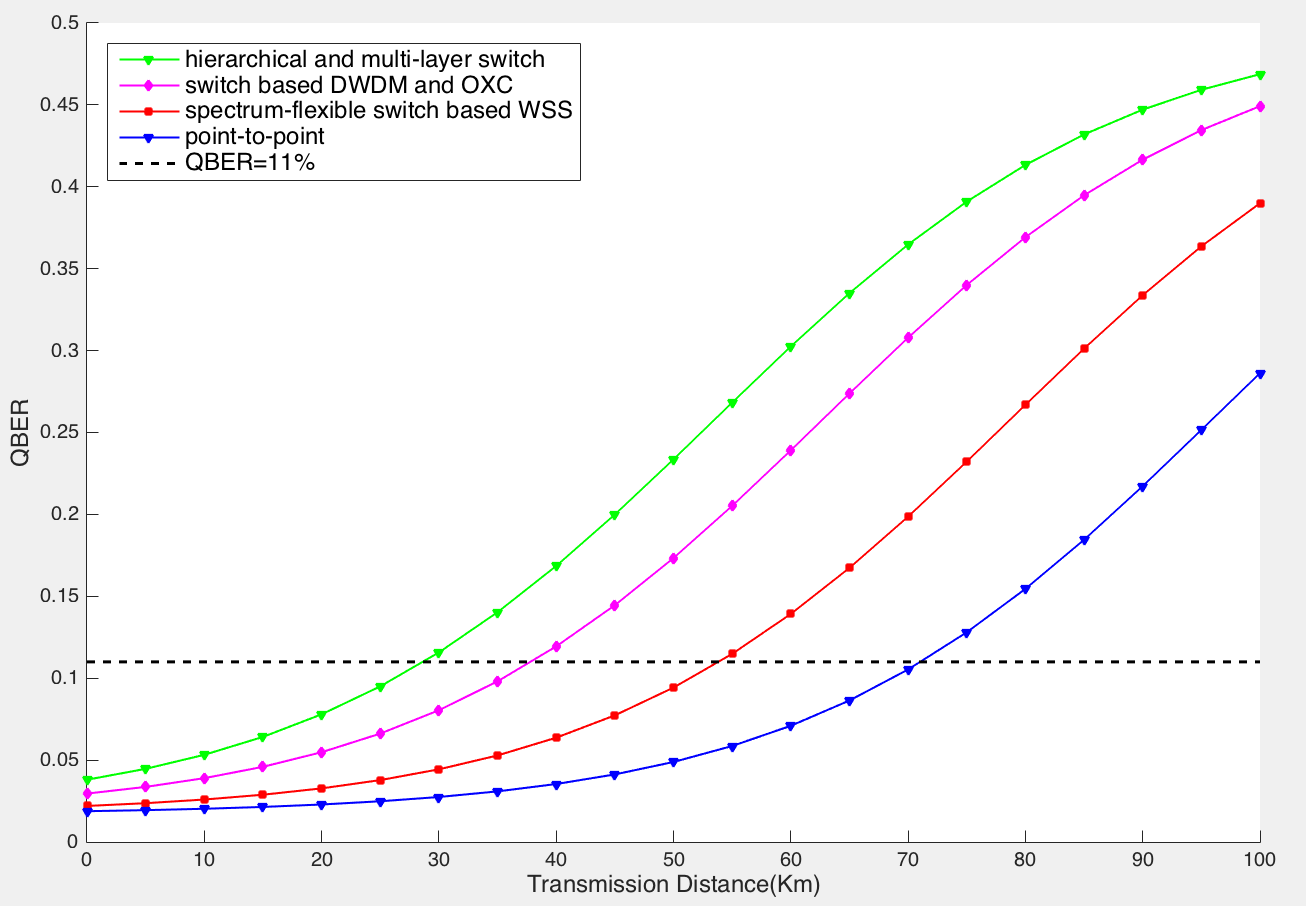
\includegraphics[height= 4cm,width=.9\linewidth]{distance_of_transmission_with_label}
     \caption{Transmission Distance vs QBER} 
     \label{Fig:distance_vs_qber}
   \end{minipage}
\end{figure}

\section{Experiment setup}
Our experimental implementation, as figure \ref{Fig:experiment_of_switching_node} shows, is composed of quantum transmitter/receiver, optical transmitter/receiver and the switching node.
\begin{figure}
 \centering
 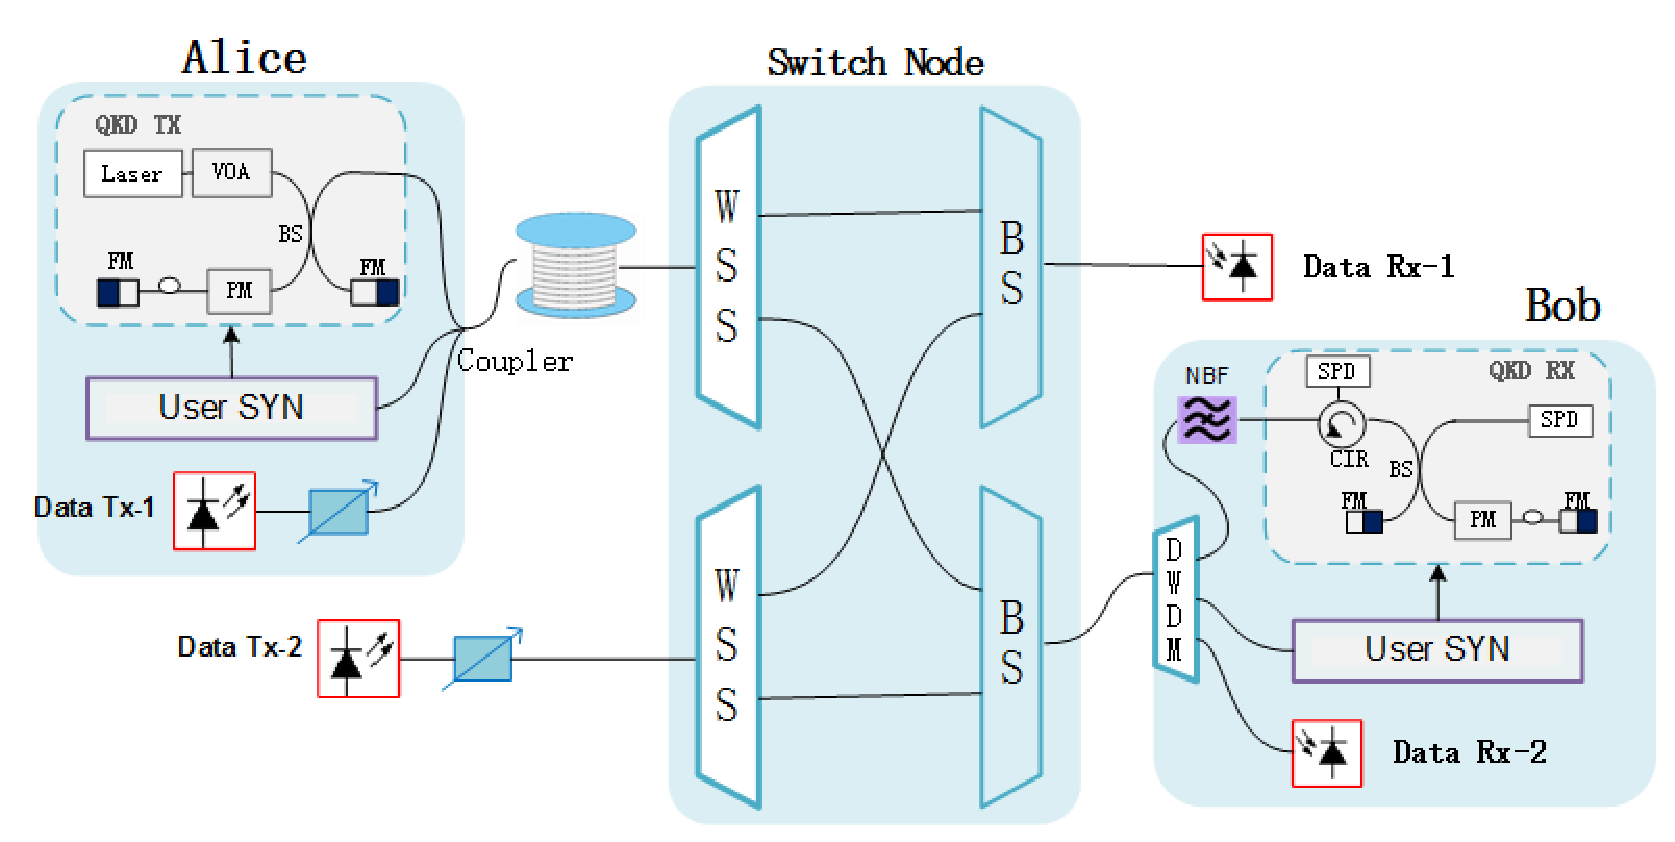
\includegraphics[height= 4cm,width=.6\linewidth]{experiment_of_switching_node}
 \caption{Experiment setup based Coexistence Switching Node}
 \label{Fig:experiment_of_switching_node}
\end{figure}
Alice has ability to send the quantum signal, quantum sync signal and classic signal. Bob could receive and demodulate these three kinds of signals. QKD transmitter consists of pulsed light source (LS), splitter, faraday mirror(FM) and Faraday-Michelson interferences that contains phase modulator (PM). QKD receiver has the signal photon detector(SPD). Since it is difficult to create true single photon pulses, a pulsed 1553.73nm laser diode (1-ns pulse width) with 10MHz repetition rate is followed by variable optical attenuator(VOA) to approximate single photon generation. In order to detect the quantum signal in the appropriate time, we need a signal to synchronize the time of detection and set it's center wavelength 1529.99nm. There are two 1550nm Optical waves for sending large data as text, image, video etc. When performing quantum communication, there is amount of base selection information needed to be sent on the public network. Since the switching node is unidirectional, if we make the public network go through the quantum switching node and switched by switching node, we need to build two switch nodes. In cost consideration, we build another public network without switching node that connect Alice and Bob directly. In this experiment, we set up three sets of contrast experiments: (a) Point-to-point quantum communication experiment; (b) Only quantum communication passes through the switching node; (c) Quantum and classic communication pass through the switching node at the same time.

\begin{figure}[!htb]
   \begin{minipage}{0.48\textwidth}
     \centering
     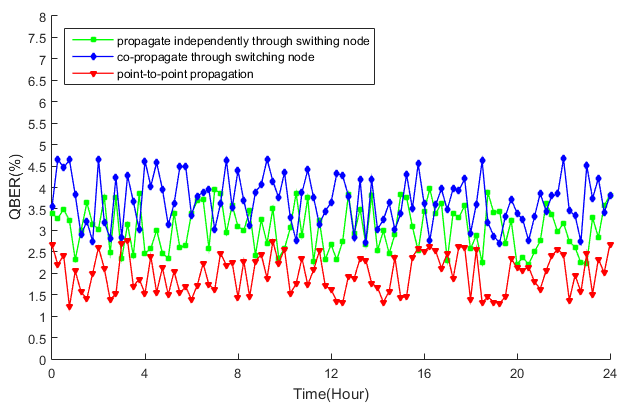
\includegraphics[width=.9\linewidth]{qber_experiment}
     \caption{QBER performance for 24 hours} \label{Fig:comparison_of_loss}
   \end{minipage}\hfill
   \begin{minipage}{0.48\textwidth}
     \centering
     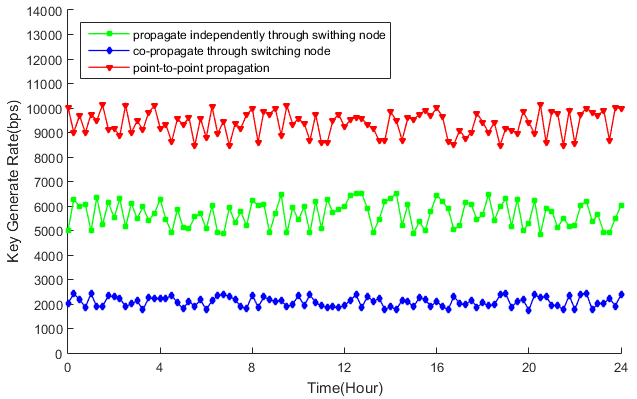
\includegraphics[width=.9\linewidth]{key_rate_experiment}
     \caption{Key Generation Rates performance for 24 hours} \label{Fig:comparison_of_rate}
   \end{minipage}
\end{figure}
Figure \ref{Fig:comparison_of_loss} and \ref{Fig:comparison_of_rate} show the system performance of continuous 24 hours operation. the result shows that the co-propagation switching could be realized by this switching node, and the quantum bit error rate(QBER) and key generation rate(KGR) is acceptable. In point-to-point situation, the average QBER is 1.7\%, and average KGR is 9000bps. In co-propagation situation, the average QBER is 3.7\%, and average KGR is 2300bps. Although performance declines, it is still acceptable.

\section{Conclusions}
We have an experiment on flattened and  and Spectrum-flexible switching node with co-propagation of quantum and optical signal. This architecture supports flexible spectrum and bandwidth allocation and has ability to switch signals mixed of quantum signal and optical signal.
%%We proposed a flattened flexible non-blocking switching node with quantum and classic optic coexistence, this architecture could be compatible with the switch of quantum signals and classical optical signals,  quantum communication optical network and the integration of the classic optical network to provide the basis, which provides the foundation for the integration of quantum communication optical network and classical optical network.

\section{Acknowledgements}
This work is supported in part by National Natural Science Foundation of China (Grant No. 61331008) and Science and Technology Project of State Grid Corporation of China.
%% (Research on Structure and Key Networking Technology of Quantum Secure Communication in Space-earth System)



\begin{thebibliography}{99}

\bibitem{Peters} Peters, NA and Toliver, et al. "Quantum communications in reconfigurable optical networks: DWDM QKD through a ROADM" National Fiber Optic Engineers Conference, 2010 Conference on (OFC/NFOEC). IEEE.

\bibitem{YongmeiSun} Sun, Yongmei, et al. "Reduction of FWM noise in WDM-based QKD systems using interleaved and unequally spaced channels." Chinese Optics Letters 14.6 (2016): 060602.

\bibitem{ToliverPaul} Toliver, Paul, et al. "Experimental investigation of quantum key distribution through transparent optical switch elements." IEEE Photonics Technology Letters 15.11 (2003): 1669-1671.

\bibitem{WangShuang} Wang, Shuang, et al. "Field test of wavelength-saving quantum key distribution network." Optics letters 35.14 (2010): 2454-2456.

\bibitem{NiuJianing} Niu, Jianing, et al. "A Novel Scheme of Integrating QKD in WDM-PON." Asia Communications and Photonics Conference. Optical Society of America, 2016.

\end{thebibliography}
\end{document}
